\documentclass[12pt, a4paper]{article}

% Pacotes essenciais
\usepackage[utf8]{inputenc}
\usepackage[T1]{fontenc}
\usepackage[portuguese]{babel}
\usepackage{amsmath}
\usepackage{amsfonts}
\usepackage{amssymb}
\usepackage{graphicx}
\usepackage{booktabs}
\usepackage[margin=2.5cm]{geometry}
\usepackage{setspace}
\usepackage{longtable}

% Adição do pacote natbib para citações no formato (Autor, Ano)
\usepackage[round, authoryear]{natbib}

% Configuração de links e metadados
\usepackage{hyperref}
\hypersetup{
    colorlinks=true,
    linkcolor=blue,
    filecolor=magenta,      
    urlcolor=cyan,
    citecolor=black,
}

\begin{document}

% Título e Autor com notas de rodapé (substitua os textos conforme necessário)
\title{O Impacto da Tarifa Zero no Emprego Local: Evidências para o Setor de Comércio e Serviços em Municípios de Médio Porte Brasileiros\thanks{Artigo submetido como Avaliação da Disciplina de Tópicos Especiais de Econometria}}

\author{Alexandre Bezerra dos Santos\thanks{Graduando em Ciências Econômicas pela Universidade Federal de Pernambuco}}

\date{27 de Maio de 2026}

\maketitle

% Resumo
\begin{abstract}
A adoção da política de gratuidade universal no transporte público urbano, conhecida como "Tarifa Zero", tem crescido expressivamente nos municípios brasileiros, levantando debates sobre os seus impactos que extrapolam a esfera fiscal. Este artigo tem como objetivo avaliar o impacto causal da implementação da Tarifa Zero sobre a geração de emprego formal nos setores de comércio e serviços locais. Utilizando microdados mensais do Novo Cadastro Geral de Empregados e Desempregados (Novo CAGED) no período recente, o estudo constrói um painel municipal focado em cidades de médio porte (30 a 400 mil habitantes). Em virtude da implementação defasada da política no tempo, aplica-se o estimador de Diferenças-em-Diferenças proposto por Callaway e Sant'Anna (2021), robusto à heterogeneidade temporal e espacial, contornando os enviesamentos dos modelos tradicionais de Efeitos Fixos de Duas Vias. Os resultados evidenciam um Efeito Médio do Tratamento (ATT) positivo e estatisticamente significante: a eliminação da tarifa gera, em média, 0,12 postos de trabalho adicionais por 1.000 habitantes ao mês nos setores analisados. A análise dinâmica via estudo de eventos corrobora a quebra estrutural nas tendências de contratação no período pós-tratamento. Conclui-se que a Tarifa Zero atua como um choque positivo de rendimento e reduz as fricções espaciais de procura por emprego, dinamizando a economia local e gerando externalidades positivas tangíveis para o mercado de trabalho municipal. 

\vspace{0.5cm}
\noindent \textbf{Palavras-chave:} Tarifa Zero; Mercado de Trabalho; Diferenças-em-Diferenças; Avaliação de Políticas Públicas.
\end{abstract}

\newpage

% Seção 1
\section{Introdução}
Nos últimos anos, a Tarifa Zero deixou de ser uma experiência pontual em poucos municípios para ganhar espaço no debate público e na agenda de políticas urbanas no Brasil, sobretudo após a crise do financiamento do transporte coletivo e a queda persistente da demanda por passageiros.
Essa expansão tem chamado atenção não apenas pelos seus efeitos sobre a mobilidade, mas também pelo potencial de alterar a forma como famílias e trabalhadores acessam oportunidades e circulam pela cidade \citep{sartori2023}.
Levantamentos recentes mostram que o número de cidades brasileiras com alguma forma de gratuidade no transporte coletivo cresceu rapidamente na última década, incluindo experiências integrais, parciais e restritas a determinados dias ou perfis de usuários \citep{ntu2023}.
Apesar disso, boa parte do debate ainda se concentra no custo fiscal da política e em sua sustentabilidade orçamentária, enquanto permanecem menos explorados seus possíveis efeitos sobre o emprego, o consumo local e a dinâmica econômica dos municípios \citep{sampaio2024, pereiravermanderkeblowski2023}.

Do ponto de vista econômico, há pelo menos dois caminhos pelos quais a Tarifa Zero pode produzir efeitos além da mobilidade.
O primeiro caminho passa pelo orçamento das famílias: quando uma despesa recorrente com transporte é reduzida ou eliminada, sobra renda para outras compras do dia a dia, o que tende a beneficiar especialmente os domicílios de menor renda e a fortalecer o consumo em setores voltados ao mercado local.
O segundo caminho passa pelo mercado de trabalho, pois, ao diminuir o custo de ir e vir, a política pode ampliar o raio de busca por vagas e facilitar o acesso a empregos antes pouco viáveis por causa da distância ou do gasto com deslocamento \citep{kain1968, gobilonselodzenou2007, Franklin2018}.

Essa ligação entre transporte e trabalho aparece de forma recorrente na literatura urbana e do trabalho.
A hipótese do desajuste espacial, formulada por \citet{kain1968}, sustenta que a separação entre moradia e emprego pode piorar o acesso às oportunidades, sobretudo para trabalhadores de baixa renda; estudos posteriores reforçam que custos de deslocamento e tempo de viagem funcionam como barreiras concretas à procura por trabalho e à aceitação de vagas \citep{BruecknerZenou2003, zenou2009, BastiaassemJohnsonLucas2020}.
Em termos práticos, isso significa que a gratuidade pode fazer diferença, por exemplo, para quem depende de ônibus diários para aceitar uma vaga em outra parte da cidade sem comprometer boa parte do salário líquido.

Apesar desses mecanismos serem plausíveis e bem discutidos pela teoria, ainda são escassas, no Brasil, as evidências causais sobre os efeitos da Tarifa Zero no mercado de trabalho formal e na economia local.
A literatura nacional tem avançado mais na descrição das experiências municipais, no debate sobre financiamento e nos vínculos da política com inclusão e direito à cidade do que na mensuração de seus impactos econômicos diretos.
É nesse ponto que esta pesquisa se insere, ao perguntar qual é o impacto causal da implementação da Tarifa Zero municipal sobre o saldo de empregos formais nos setores de comércio e serviços.

Para responder a essa pergunta, o trabalho combina informações sobre municípios que adotaram a Tarifa Zero integral a partir de 2020 e mantiveram a política até meados de 2026 com microdados mensais do Novo CAGED, principal fonte conjuntural sobre admissões e desligamentos formais no país.
A análise se concentra em municípios de médio porte, com população entre 30 mil e 400 mil habitantes segundo as estimativas populacionais do IBGE para 2019, o que ajuda a tornar mais comparáveis as cidades tratadas e as cidades de controle e reduz diferenças extremas de estrutura econômica e urbana.

Como a política foi implementada em momentos diferentes entre os municípios, a estratégia empírica usa um modelo de Diferenças-em-Diferenças com adoção defasada, comparando a trajetória do emprego nas cidades que passaram a adotar a medida com a de cidades semelhantes que ainda não a haviam implementado.
A literatura recente mostra que, nesses contextos, estimadores tradicionais com efeitos fixos de duas vias podem gerar comparações problemáticas quando os efeitos do tratamento variam ao longo do tempo; por isso, o estudo adota o estimador proposto por \citet{CallawaySantanna2021}, hoje amplamente usado nesse tipo de aplicação \citep{DechaisematinDhaultfoeuille2020, goodman2021, rothsantannabilinskipoe2023}.

Os resultados apontam para um efeito positivo, estatisticamente significativo e economicamente relevante da Tarifa Zero sobre o emprego formal nos setores de comércio e serviços.
Em média, as estimativas indicam um saldo adicional de cerca de 0,12 posto formal por mês a cada 1.000 habitantes nos municípios tratados, sugerindo que a política pode gerar efeitos que vão além da mobilidade e alcançar a atividade econômica local.
A análise dinâmica reforça esse resultado: após a adoção da política, a trajetória das contratações passa a se deslocar de forma mais favorável nos municípios tratados do que nos não tratados, ainda que o padrão mensal preserve a sazonalidade típica do comércio varejista e dos serviços.
Esse comportamento é compatível com a ideia de que a redução dos custos de deslocamento e o alívio no orçamento das famílias podem afetar tanto a oferta quanto a demanda de trabalho no nível local.

Além desta introdução, o trabalho está organizado em quatro seções.
A próxima seção revisa a literatura sobre custos de deslocamento, mercado de trabalho e efeitos locais da Tarifa Zero.
Em seguida, são apresentados os dados, o recorte amostral e a estratégia de identificação.
Depois, o texto discute os resultados principais, o estudo de eventos e os testes de robustez.
Por fim, a última seção reúne as considerações finais e as implicações da pesquisa para o debate sobre políticas públicas urbanas.

% Seção 2
\section{Revisão da Literatura}
Esta seção reúne os principais argumentos teóricos que ajudam a entender por que a Tarifa Zero pode produzir efeitos que vão além da mobilidade urbana.
Em vez de tratar apenas do transporte em si, a literatura mostra que essa política também pode influenciar o acesso ao trabalho e o orçamento das famílias, com possíveis reflexos sobre a atividade econômica local.
No caso brasileiro, porém, os estudos ainda têm dado mais atenção aos desafios de financiamento, à implementação institucional e aos efeitos sobre a circulação urbana.
Com isso, ainda são limitadas as análises que investigam de forma mais direta como a política pode afetar o emprego e a dinâmica econômica dos municípios.

\subsection{Fricções de Procura e a Hipótese de Desajuste Espacial}
Na economia urbana, uma ideia bastante consolidada é que o custo e o tempo de deslocamento podem dificultar a inserção no mercado de trabalho, porque reduzem o acesso efetivo às vagas e tornam a procura por emprego mais cara e mais demorada \citep{gobilonselodzenou2007, BastiaassemJohnsonLucas2020}.
Esse argumento ganhou forma clássica com a Hipótese do Desajuste Espacial (\textit{Spatial Mismatch Hypothesis}), associada ao trabalho pioneiro de \citet{kain1968}, segundo a qual a distância entre onde os trabalhadores moram e onde os empregos se concentram pode piorar os resultados no mercado de trabalho.

Em geral, quando moradia e emprego ficam muito separados, surgem barreiras de acesso que podem elevar o desemprego, reduzir a participação e empurrar parte dos trabalhadores para ocupações mais precárias, especialmente entre grupos de menor renda \citep{BruecknerZenou2003, wangwuchao2022}.
No caso brasileiro, esse problema tende a ser mais forte porque uma parcela importante da população trabalhadora vive em áreas periféricas, enquanto muitas oportunidades formais seguem concentradas em regiões mais centrais e mais bem conectadas, o que aprofunda desigualdades de acesso ao trabalho \citep{silvaporsse2024, reisveras2024}.

Nos modelos de procura por trabalho (\textit{Search and Matching}), a passagem diária entre casa e emprego entra como um custo concreto da decisão de trabalhar, pois, quanto maior o gasto com tarifa, tempo e conexões, maior tende a ser o salário-mínimo que a pessoa considera aceitável para sair da busca e assumir uma vaga, o que a literatura denomina por salário de reserva \citep{vandenberggorter2022, zenou2009}.
Em termos práticos, isso ajuda a entender por que uma vaga de atendente, caixa ou auxiliar de serviços, embora exista, pode não ser viável para quem mora longe e precisa gastar parte relevante do rendimento só para chegar ao trabalho, esmagando o salário de reserva líquido.

\citet{zenou2009} enfatiza esse mecanismo teórico, ao mostrar como os custos de deslocamento afetam a aceitação das ofertas; já \citet{Franklin2018}, com evidência experimental para jovens em Addis Ababa, mostra que subsídios de transporte aumentam a intensidade da procura e a chance de conseguir empregos melhores, sugerindo que a barreira não é apenas espacial, mas também financeira.
Essa discussão conversa com revisões mais amplas, como a de \citet{BastiaassemJohnsonLucas2020}, que encontram evidências majoritariamente positivas da relação entre transporte e acesso ao emprego, embora ressaltem que os efeitos variam conforme o desenho da política e o contexto urbano.

Em mercados locais como comércio e serviços, onde são comuns postos de entrada, salários mais baixos e alta rotatividade, esse custo pesa ainda mais, porque pequenas despesas de deslocamento podem decidir se vale ou não aceitar a vaga.
Quando a tarifa é reduzida ou eliminada, o trabalhador pode ampliar o raio de busca e considerar empregos antes descartados por serem distantes ou pouco vantajosos no curto prazo, o que tende a melhorar o encaixe entre quem procura trabalho e as oportunidades disponíveis \citep{gobilonselodzenou2007, Flemming2020}.
Ou seja, a instituição da gratuidade universal, pode promover mudanças na distribuição espacial das atividades econômicas dos municípios que a adotam.

\subsection{Efeito Renda e o Multiplicador Local}
Pelo lado da demanda local, a eliminação da tarifa funciona como um alívio imediato no orçamento das famílias que dependem do transporte público, porque reduz uma despesa recorrente e libera renda para outros usos \citep{proquebetarellijuniorribeiro2024, CrawleyTheloudis2024}.
No caso brasileiro, esse ponto é especialmente importante porque o gasto com transporte ocupa uma parcela relevante do orçamento doméstico e pesa relativamente mais sobre os grupos de menor renda, para os quais pequenas economias no mês podem fazer diferença concreta no consumo cotidiano \citep{ibge2020, proquebetarellijuniorribeiro2024}.

Na prática, isso significa que o valor antes gasto com passagem pode ser redirecionado para compras em supermercados, farmácias, contas básicas ou pequenos serviços do bairro, o que ajuda a sustentar a atividade de setores voltados ao consumo local, de bens e serviços não transacionáveis.
Esse raciocínio se aproxima da literatura sobre choques de renda e consumo das famílias, que mostra que ganhos de renda, sobretudo entre famílias com orçamento apertado, tendem a ser rapidamente transformados em gasto corrente \citep{CrawleyTheloudis2024}.

Ao mesmo tempo, estudos sobre efeitos econômicos locais ajudam a entender por que esse movimento pode ir além do orçamento de cada família.
\citet{moretti2010} mostra que choques de demanda e emprego em uma economia local costumam se espalhar para setores voltados ao mercado interno, especialmente comércio e serviços, porque esses segmentos respondem diretamente ao aumento do gasto das famílias.
Em diálogo com esse argumento, \citet{GerardNaritomiSilva2021} encontram evidências para o caso brasileiro de que transferências de renda podem ativar a economia municipal ao elevar o consumo e estimular atividades não transacionáveis, isto é, aquelas que dependem do gasto feito dentro da própria cidade.

Na prática, isso ajuda a explicar por que, quando muitas famílias passam a economizar com transporte ao mesmo tempo, parte desse valor pode reaparecer em refeições fora de casa, compras em mercadinhos, salões de beleza, farmácias, oficinas e outros serviços de bairro.
Quando esse aumento de demanda se distribui por vários estabelecimentos ao mesmo tempo, as firmas tendem a ajustar escala, horário de funcionamento e uso da mão de obra, o que pode abrir espaço para novas contratações, sobretudo em atividades com alta rotatividade e forte dependência do consumo cotidiano \citep{moretti2010, GerardNaritomiSilva2021}.

Assim, a gratuidade no transporte pode produzir um efeito econômico indireto que não se limita à mobilidade: ao aliviar um gasto recorrente e ampliar a circulação de renda dentro do município, ela também pode reforçar a atividade local e sustentar o emprego em setores mais sensíveis à demanda das famílias.
Esse mecanismo tende a ser especialmente visível em centros comerciais e áreas com forte presença de serviços presenciais, onde um aumento mesmo modesto no fluxo de consumidores pode elevar a procura efetiva e pressionar as empresas a reforçar equipes de atendimento, reposição, entrega ou operação.
Em termos simples, mais gente circulando e consumindo no comércio local pode significar mais horas de trabalho e, em alguns casos, novas vagas formais, principalmente em negócios pequenos e médios que reagem rapidamente às oscilações da demanda \citep{moretti2010, GerardNaritomiSilva2021}.

\subsection{Evidência Empírica e a Lacuna Metodológica}
Apesar de os mecanismos teóricos estarem relativamente bem estabelecidos, ainda são poucos os estudos que conseguem medir com clareza o efeito causal da Tarifa Zero sobre emprego e atividade econômica local.
No cenário internacional, a evidência mais próxima costuma vir de políticas mais focalizadas, como passes subsidiados para desempregados ou gratuidades temporárias para grupos específicos, e não de sistemas universais e permanentes de gratuidade.
\citet{phillips2014}, por exemplo, mostra que reduzir o custo do transporte pode aumentar a intensidade da busca por trabalho entre pessoas de baixa renda; já \citet{Franklin2018} encontra que subsídios de transporte elevam a procura e melhoram a chance de alcançar empregos de melhor qualidade.

Esses resultados apontam na mesma direção, mas também sugerem cautela.
Eles ajudam a entender por que o transporte importa para o mercado de trabalho, sem resolver completamente o que acontece quando a política é adotada em escala municipal e para toda a população usuária.
No Brasil, a literatura ainda tem avançado mais pelo lado institucional, normativo e descritivo do que pela mensuração causal de resultados econômicos.

Estudos recentes sobre a Tarifa Zero têm se concentrado, em geral, nas motivações de implementação, nos desafios de financiamento, na relação com o direito à cidade e nos efeitos percebidos sobre inclusão e mobilidade \citep{pereiravermanderkeblowski2023, sartori2023, sampaio2024}.
Em termos práticos, isso significa que já sabemos mais sobre como os municípios viabilizam a política e por que ela ganha apoio social do que sobre seu impacto efetivo em variáveis como emprego formal, renda local ou dinamismo do setor de serviços.
É justamente nessa lacuna que este trabalho se insere.

O presente estudo se diferencia ao tratar a expansão recente da Tarifa Zero em municípios de médio porte como uma oportunidade de análise quase-natural, já que a política não foi adotada ao mesmo tempo em todos os lugares, nem sob condições idênticas.
Na prática, isso significa comparar municípios que implementaram a medida em momentos diferentes com outros semelhantes que ainda não a haviam adotado, o que ajuda a reconstruir com mais clareza o que teria acontecido com o emprego formal na ausência da política.

Essa estratégia dialoga com a literatura recente de Diferenças-em-Diferenças em contextos de adoção defasada, que mostra que estimadores tradicionais com efeitos fixos de duas vias podem misturar comparações inadequadas quando os efeitos do tratamento variam entre grupos e ao longo do tempo \citep{DechaisematinDhaultfoeuille2020, goodman2021}.
Em resposta a esse problema, \citet{CallawaySantanna2021} propõem uma forma de estimar efeitos por grupo e período, preservando comparações mais limpas entre tratados e controles válidos; já \citet{rothsantannabilinskipoe2023} sintetizam esse avanço metodológico e destacam o porquê de ele se tornar central em aplicações empíricas recentes.

Ao utilizar microdados mensais do emprego formal e esse conjunto de ferramentas, o trabalho busca medir de forma mais confiável o efeito causal da Tarifa Zero sobre o emprego local, reduzindo o risco de atribuir à política variações que, na verdade, decorreriam da composição das comparações ou do momento em que cada município entrou no tratamento.

% Seção 3
\section{Metodologia}
\subsection{Dados e Construção da Amostra}
Para investigar o impacto da adoção da Tarifa Zero sobre a dinâmica do mercado de trabalho local, o estudo constrói um painel municipal mensal com informações entre janeiro de 2020 e meados de 2026. A variável de resultado é obtida a partir do Novo Cadastro Geral de Empregados e Desempregados (Novo CAGED), base administrativa do Ministério do Trabalho e Emprego que registra admissões e desligamentos formais em alta frequência e com ampla cobertura territorial, o que a torna especialmente útil para acompanhar mudanças de curto prazo no emprego formal em nível municipal \citep{Brasil2026}.

Em desenhos quase-experimentais aplicados a políticas públicas, o uso de painéis administrativos com periodicidade mensal é valioso justamente porque permite observar com mais precisão o momento da intervenção e a trajetória do ajuste no período posterior ao tratamento \citep{FredrikssonOliveira2019, BakerCallawayCunninghamGoodmanSantanna2025}.
A análise se concentra em setores mais expostos ao fluxo local de consumidores e ao consumo de proximidade, isto é, atividades em que uma eventual economia com transporte pode aparecer com mais rapidez na forma de maior circulação, gasto e contratação.
Por isso, os microdados foram filtrados para isolar as seções de Comércio (CNAE G) e de Alojamento e Alimentação (CNAE I), segmentos em que o desempenho do emprego tende a responder mais diretamente a variações da demanda local.

Para reduzir a influência do porte populacional sobre o volume absoluto de admissões e desligamentos, a variável dependente é expressa como saldo líquido de empregos formais por 1.000 habitantes.
Essa padronização melhora a comparabilidade entre municípios de tamanhos distintos e segue uma prática comum em estudos comparativos com unidades heterogêneas, especialmente quando o interesse está na intensidade relativa do efeito, e não apenas em magnitudes absolutas \citep{imbens2004, FredrikssonOliveira2019}.

A variável de tratamento corresponde ao mês de início da gratuidade universal no transporte coletivo em cada município.
Essa informação foi construída manualmente a partir do cruzamento entre o relatório Brazilian municipalities with full Fare-Free Public Transport policies - updated September 2025, derivado do trabalho de \citet{santini2024} e atualizado em 2025, e a verificação direta em leis municipais, decretos e publicações em diários oficiais.
Esse procedimento busca reduzir erros de classificação sobre a data efetiva de adoção, um ponto sensível em avaliações com tratamento escalonado, já que pequenas imprecisões na data de entrada podem contaminar a identificação dos efeitos dinâmicos e das comparações entre grupos tratados e controles \citep{CallawaySantanna2021, rothsantannabilinskipoe2023}.

Para ampliar a comparabilidade entre municípios tratados e não tratados e preservar uma condição mínima de suporte comum, a amostra foi restrita a cidades com população entre 30 mil e 400 mil habitantes.
Com isso, foram excluídos tanto municípios muito pequenos, cuja estrutura produtiva e escala do mercado de trabalho tendem a ser bastante específicas, quanto grandes centros urbanos, onde a complexidade econômica e a oferta de transporte coletivo seguem outra lógica.
O critério de corte foi definido com base nas estimativas populacionais do IBGE para 2019, isto é, antes do início do período de tratamento.
O uso de uma característica observável medida em período estritamente pré-tratamento ajuda a evitar que a própria política influencie a composição da amostra e torna a regra de seleção mais defensável do ponto de vista da identificação, em linha com a recomendação de que decisões de desenho e comparabilidade sejam ancoradas em informações anteriores à intervenção \citep{imbens2004, FredrikssonOliveira2019, BakerCallawayCunninghamGoodmanSantanna2025}.

\subsection{Estratégia de Identificação}
A estratégia de identificação explora a variação espacial e temporal na adoção da Tarifa Zero entre os municípios da amostra.
Se todas as cidades tratadas tivessem implementado a política no mesmo momento, um modelo tradicional de Diferenças-em-Diferenças seria suficiente para comparar o antes e o depois entre tratados e controles.
Neste estudo, porém, a adoção é defasada no tempo (staggered adoption): alguns municípios entram no tratamento antes, outros depois, e isso exige um desenho que preserve comparações válidas entre grupos ao longo do período analisado \citep{CallawaySantanna2021, BakerCallawayCunninghamGoodmanSantanna2025}.

A literatura econométrica recente mostrou que, nesse tipo de contexto, o estimador tradicional com Efeitos Fixos de Duas Vias (Two-Way Fixed Effects, TWFE) pode produzir estimativas de difícil interpretação quando os efeitos do tratamento variam entre coortes ou mudam com o tempo.
O ponto central é que o TWFE tende a combinar várias comparações 2×2 implícitas, inclusive usando unidades já tratadas como grupo de controle para unidades recém-tratadas, o que pode gerar ponderações negativas e distorcer o efeito agregado \citep{DechaisematinDhaultfoeuille2020, goodman2021}.
Em termos práticos, isso significa que o coeficiente final pode refletir uma média contaminada por comparações que não correspondem ao contrafactual que se deseja estimar.

Para contornar esse problema, o estudo adota o estimador proposto por \citet{CallawaySantanna2021}, desenvolvido para painéis com adoção defasada.
Em vez de resumir todo o efeito em um único coeficiente potencialmente enviesado, essa abordagem estima efeitos médios de tratamento específicos para cada coorte de adoção $g$ e para cada período $t$, o que torna mais transparente o que está sendo comparado e em que momento.
O parâmetro central é o efeito médio do tratamento sobre os tratados para o grupo que adota a política no período $g$ e no tempo $t$ , denotado por $ATT\left(g,t\right)$, conforme:

\begin{equation}
ATT(G,T)=\mathbb{E}[Y_t(g)-Y_t(0)|G=g]
\end{equation}

Nessa notação, $Y_t\left(g\right)$ representa o saldo de empregos no mês $t$ para os municípios que passaram a adotar a política no período $g$, enquanto $Y_t(0)$ corresponde ao resultado contrafactual esperado para esses mesmos municípios caso não tivessem sido tratados.
Neste trabalho, esse contrafactual é construído com base em um grupo de controle limpo, formado apenas por municípios da amostra que não adotaram a Tarifa Zero na janela observada (never-treated).
Essa escolha evita comparar unidades tratadas com outras que já estavam expostas à política e segue a recomendação metodológica de privilegiar grupos de controle que preservem interpretações mais claras dos efeitos por coorte e período \citep{CallawaySantanna2021, BakerCallawayCunninghamGoodmanSantanna2025}.

Para examinar como o efeito evolui ao longo do tempo, os efeitos estimados são agregados em formato de estudo de eventos (event study).
Esse exercício é útil por duas razões: ele permite observar se o impacto aparece de forma imediata ou gradual após a adoção e oferece uma verificação empírica da hipótese de tendências paralelas.
Em particular, espera-se que os coeficientes associados aos períodos anteriores ao tratamento permaneçam próximos de zero e sem significância estatística sistemática.
A literatura recente, porém, alerta que a leitura de gráficos dinâmicos em contextos de adoção defasada exige cuidado, já que especificações tradicionais com leads e lags em TWFE podem produzir aparentes pré-tendências mesmo quando o problema decorre apenas de heterogeneidade dos efeitos; por isso, a interpretação do estudo de eventos aqui segue o mesmo arcabouço de identificação adotado para os $ATT\left(g,t\right)$ \citep{sunabraham2021, CallawaySantanna2021, marcussantanna2021}.

% Seção 4
\section{Resultados e Discussão}
\subsection{O Impacto Médio Global (Overall ATT)}
A avaliação empírica indica que a adoção da Tarifa Zero produziu um impacto causal positivo e estatisticamente significativo sobre o emprego formal nos setores de comércio e serviços dos municípios analisados.
Com base no estimador de Diferenças-em-Diferenças para adoção defasada de \citet{CallawaySantanna2021}, o Efeito Médio do Tratamento sobre os Tratados (Overall ATT) foi estimado em 0,1234, com erro-padrão de 0,0400.
Esse coeficiente é estatisticamente significativo ao nível de 5\%, com intervalo de confiança de 95\% entre 0,0450 e 0,2018.

Mais do que significante em termos estatísticos, o resultado também tem relevância econômica.
Em termos práticos, a estimativa sugere que a política está associada à criação líquida média de cerca de 0,12 posto formal por mês para cada 1.000 habitantes.
Em um município típico da amostra com 100 mil habitantes, isso corresponde a aproximadamente 12 vínculos formais adicionais por mês nos setores de comércio e serviços de proximidade, já descontadas as variações comuns do ambiente macroeconômico e das tendências agregadas observadas no período.

\subsection{Dinâmica Temporal e Estudo de Eventos}
Para examinar como o efeito da Tarifa Zero evolui ao longo do tempo e, ao mesmo tempo, avaliar a consistência da estratégia de identificação, os efeitos estimados foram organizados em formato de estudo de eventos (event study).
A Figura 1 resume essa trajetória dinâmica, enquanto a Tabela 1, no Apêndice, apresenta os coeficientes estimados com maior detalhamento.
Esse tipo de exercício é importante porque permite observar não apenas se há impacto médio após a adoção da política, mas também quando esse efeito começa a aparecer, como ele se comporta nos períodos seguintes e se o padrão pré-tratamento é compatível com a hipótese de tendências paralelas.

No período pré-tratamento ($t<0$), os coeficientes oscilam em torno de zero, embora alguns pontos específicos apareçam com maior volatilidade e significância pontual.
Esse comportamento exige cautela, mas não compromete, por si só, a interpretação do modelo.
Como a variável de resultado é construída com dados mensais do Novo CAGED, parte dessa oscilação reflete a sazonalidade própria dos setores analisados, especialmente do comércio varejista, que costuma concentrar contratações no fim do ano e ajustes no início do ano seguinte.
Além disso, mesmo com a restrição amostral por porte populacional, os municípios tratados e de controle ainda podem apresentar diferenças residuais na composição produtiva e no calendário local de atividade econômica, o que torna mais difícil suavizar completamente choques sazonais assimétricos em janelas mensais.

Ainda assim, o padrão geral do gráfico é informativo porque a trajetória estimada muda de forma perceptível após a entrada no tratamento.
Esse ponto é importante: o estudo de eventos não substitui a estimativa agregada do Overall ATT, mas ajuda a mostrar de que maneira esse efeito médio se forma ao longo do tempo.
Em vez de sugerir um salto isolado e transitório, a evidência visual indica uma inflexão consistente na trajetória dos municípios tratados, em linha com a ideia de que os efeitos da política se acumulam à medida que famílias e firmas ajustam seu comportamento no período posterior à implementação.

\begin{figure}[h!]
    \centering
    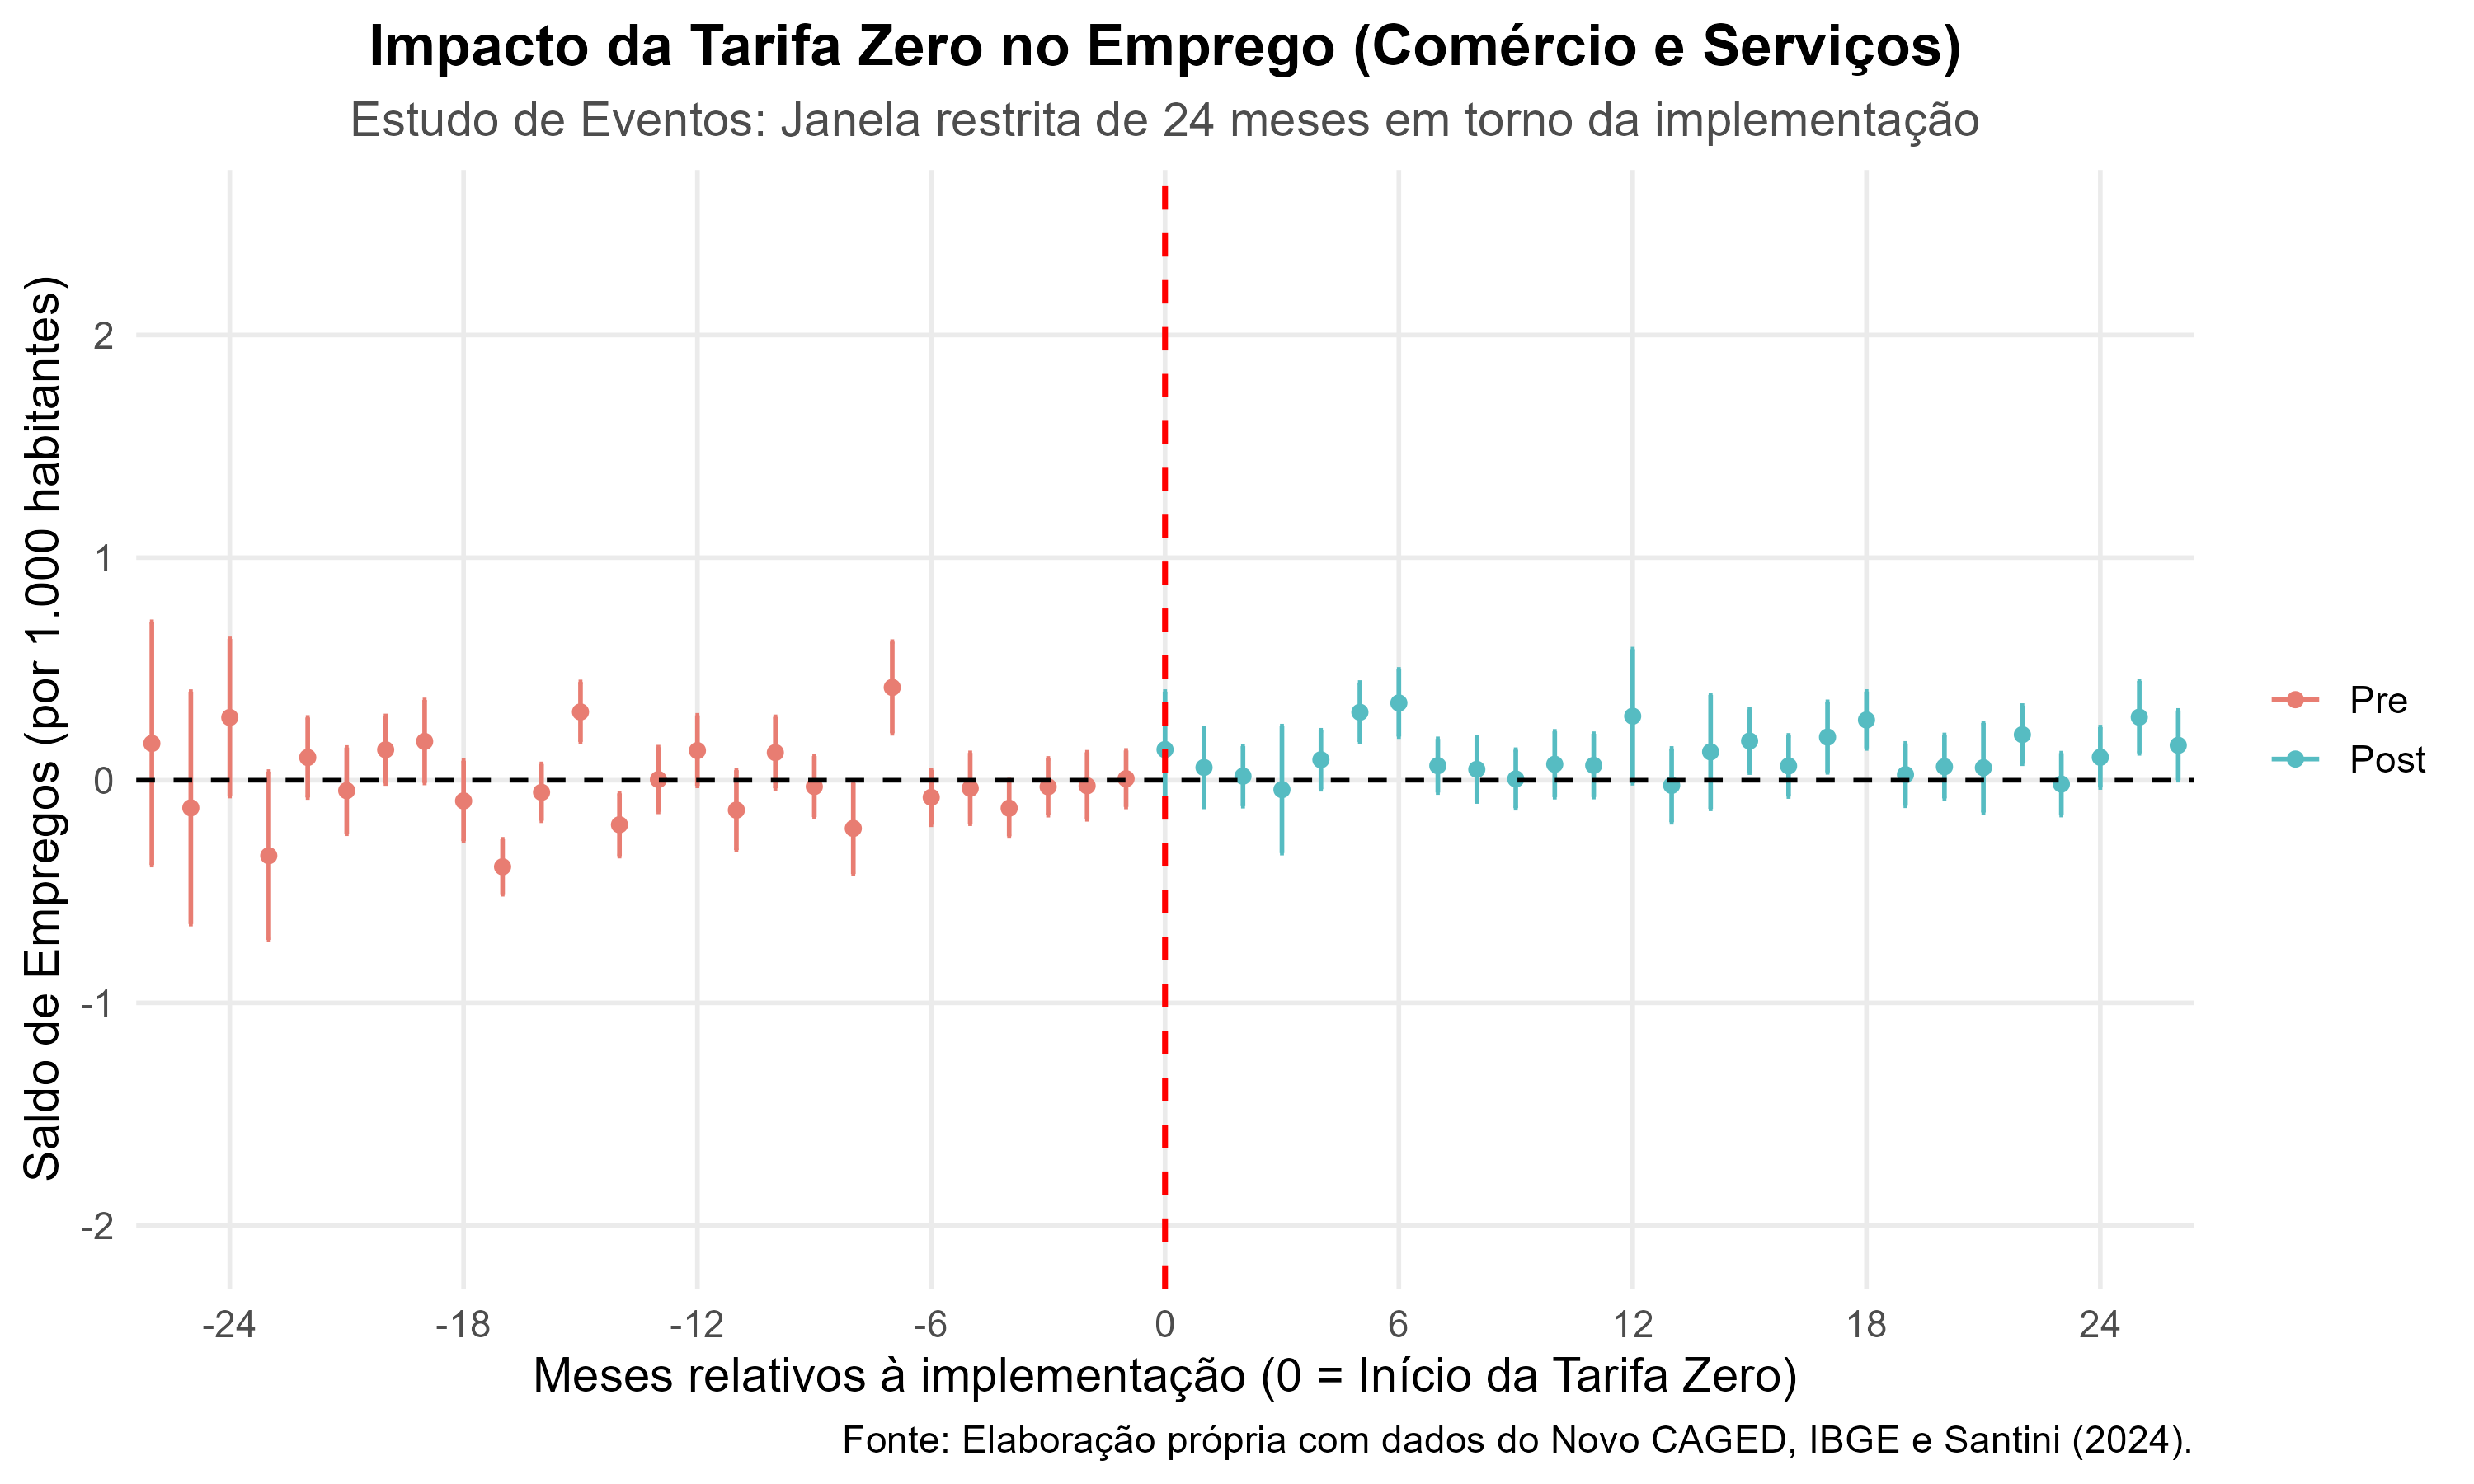
\includegraphics[width=0.8\textwidth]{graficos/Grafico_Evento_TarifaZero.png}
    \caption{Impacto da Tarifa Zero no Emprego (Comércio e Serviços)}
    \label{fig:1}
\end{figure}

No período imediatamente posterior à implementação da medida ($t >= 0$), observa-se uma mudança mais nítida no comportamento dos coeficientes, que passam a assumir valores predominantemente positivos e se afastam do nível de base.
Essa inflexão é compatível com a interpretação de que a Tarifa Zero produz efeitos relativamente rápidos sobre a economia local.
De um lado, a redução dos custos de deslocamento pode aliviar o orçamento das famílias e ampliar o gasto em comércio e serviços de proximidade, reforçando a demanda local.
De outro, a queda no custo de acesso ao trabalho pode reduzir barreiras à aceitação de vagas e facilitar o matching entre trabalhadores e postos disponíveis, especialmente em atividades com alta rotatividade e forte dependência de presença física.

Assim, a dinâmica estimada pelo estudo de eventos reforça a leitura substantiva do resultado principal: mais do que um efeito pontual, a política parece estar associada a um deslocamento persistente da trajetória do emprego formal nos setores mais sensíveis à circulação urbana e ao consumo cotidiano.

% Seção 5
\section{Considerações Finais}
Este estudo buscou preencher uma lacuna empírica ainda relevante na literatura brasileira sobre Tarifa Zero ao estimar seu efeito causal sobre o mercado de trabalho local em municípios de médio porte.
Ao explorar a variação espaço-temporal na adoção da política e utilizar o estimador de Diferenças-em-Diferenças de \citet{CallawaySantanna2021}, o trabalho procurou isolar com mais precisão o impacto da gratuidade universal do transporte coletivo sobre o saldo de empregos formais nos setores de comércio e serviços, reduzindo os problemas de comparação associados aos modelos tradicionais com efeitos fixos de duas vias \citep{DechaisematinDhaultfoeuille2020, goodman2021, rothsantannabilinskipoe2023}.

Os resultados apontam para um efeito positivo, estatisticamente significativo e economicamente relevante da Tarifa Zero sobre o emprego formal local.
Esse achado dialoga diretamente com os mecanismos discutidos ao longo do trabalho.
Pelo lado da oferta de trabalho, ele é compatível com a literatura sobre desajuste espacial e custos de procura, segundo a qual barreiras de deslocamento reduzem o acesso efetivo às vagas, elevam o custo da busca e dificultam o encaixe entre trabalhadores e empregos \citep{kain1968, gobilonselodzenou2007, zenou2009}.
Pelo lado da demanda, os resultados também conversam com a literatura sobre efeito-renda e multiplicadores locais, que mostra como alívios orçamentários e choques de renda podem se converter em maior consumo de bens e serviços não transacionáveis e, por essa via, sustentar emprego em atividades voltadas ao mercado interno \citep{moretti2010, GerardNaritomiSilva2021, CorbiPapaionnouSurico2019}.

Em conjunto, a evidência encontrada sugere que a Tarifa Zero não atua apenas como política de mobilidade ou como instrumento associado ao direito à cidade, mas também como uma intervenção com efeitos econômicos mensuráveis sobre a dinâmica do emprego urbano.
Esses resultados trazem implicações importantes para o debate sobre políticas públicas urbanas.
No Brasil, a discussão sobre Tarifa Zero ainda costuma se concentrar no custo fiscal imediato e na sustentabilidade orçamentária dos municípios, como mostram estudos recentes sobre financiamento e implementação da política \citep{pereiravermanderkeblowski2023, sampaio2024}.

Os achados deste trabalho sugerem, porém, que essa lente é incompleta quando ignora os efeitos indiretos da política sobre atividade econômica, emprego e circulação de renda no território.
Esse ponto se aproxima do debate mais amplo sobre multiplicadores locais: quando uma política altera o orçamento das famílias ou reduz uma fricção relevante para o acesso ao trabalho, seus efeitos podem se espalhar para o comércio, os serviços e, em alguma medida, para a própria arrecadação futura, ainda que isso não elimine a necessidade de discutir formas estáveis de financiamento.
Em outras palavras, a evidência aqui apresentada não autoriza tratar a Tarifa Zero como uma política sem custo, mas indica que avaliá-la apenas como despesa pública provavelmente subestima parte relevante de seus efeitos econômicos.

Ao mesmo tempo, os resultados devem ser interpretados à luz das limitações do estudo.
O uso de dados mensais do Novo CAGED permite acompanhar com precisão a resposta de curto prazo do emprego formal, mas também introduz maior volatilidade e sazonalidade, especialmente em setores como comércio e alimentação, o que dificulta uma leitura perfeitamente linear das trajetórias pré-tratamento.
Além disso, o horizonte temporal observado ainda é relativamente curto para responder se os efeitos estimados persistem no longo prazo, se se traduzem em mudanças salariais ou se alteram a composição setorial do emprego.

Por isso, uma agenda de pesquisa futura pode avançar em pelo menos três direções.
A primeira é combinar o desenho aqui utilizado com bases anuais mais consolidadas, como a RAIS, que permitem acompanhar vínculos formais com maior estabilidade temporal e maior detalhamento ocupacional.
A segunda é investigar mecanismos com mais profundidade, distinguindo melhor os canais de oferta de trabalho, demanda local e formalização.
A terceira é aproximar a avaliação econômica da discussão sobre desenho institucional da política, financiamento e heterogeneidade entre municípios, tema que ainda aparece mais forte na literatura descritiva do que na causal \citep{phillips2014, Franklin2018, pereiravermanderkeblowski2023}.

Mesmo com essas limitações, o estudo oferece uma evidência inicial robusta de que a gratuidade universal do transporte coletivo pode produzir efeitos que ultrapassam a esfera da mobilidade e alcançam, de forma concreta, o funcionamento da economia urbana local.

\newpage

% Referências
\renewcommand{\refname}{\centering{Referências Bibliográficas}}
\begin{thebibliography}{99}

\bibitem[NTU(2025)]{ntu2025}
ASSOCIAÇÃO NACIONAL DAS EMPRESAS DE TRANSPORTES URBANOS. \textit{Tarifa zero nas cidades do Brasil}. Brasília: NTU/FGV Transportes, 2025.

\bibitem[Baker et al.(2025)]{BakerCallawayCunninghamGoodmanSantanna2025}
BAKER, A.; CALLAWAY, B.; CUNNINGHAM, S.; GOODMAN-BACON, A.; SANT’ANNA, P. H. C. \textit{Difference-in-differences designs: a practitioner’s guide}. Journal of Economic Literature, forthcoming, 2025.

\bibitem[Bastiaanssen, Johnson e Lucas(2020)]{BastiaassemJohnsonLucas2020}
BASTIAANSSEN, J.; JOHNSON, D.; LUCAS, K. \textit{Does transport help people to gain employment? A systematic review and meta-analysis of the empirical evidence}. Transport Reviews, v. 40, n. 5, p. 607-628, 2020.

\bibitem[Brasil(2026)]{Brasil2026}
BRASIL. Ministério do Trabalho e Emprego. \textit{Programa de Disseminação das Estatísticas do Trabalho (PDET): Novo CAGED}. Brasília: MTE, 2026.

\bibitem[Brueckner e Zenou(2003)]{BruecknerZenou2003}
BRUECKNER, J. K.; ZENOU, Y. \textit{Space and unemployment: the labor-market effects of spatial mismatch}. Journal of Labor Economics, v. 21, n. 1, p. 242-266, 2003.

\bibitem[Callaway e Sant'Anna(2021)]{CallawaySantanna2021}
CALLAWAY, B.; SANT’ANNA, P. H. C. \textit{Difference-in-differences with multiple time periods}. Journal of Econometrics, v. 225, n. 2, p. 200-230, 2021.

\bibitem[Corbi, Papaioannou e Surico(2019)]{CorbiPapaionnouSurico2019}
CORBI, R.; PAPAIOANNOU, E.; SURICO, P. \textit{Regional transfer multipliers}. Review of Economic Studies, v. 86, n. 5, p. 1901-1934, 2019.

\bibitem[Crawley e Theloudis(2024)]{CrawleyTheloudis2024}
CRAWLEY, E.; THELOUDIS, A. \textit{Income shocks and their transmission into consumption}. Finance and Economics Discussion Series. Washington, D.C.: Board of Governors of the Federal Reserve System, 2024.

\bibitem[de Chaisemartin e D'Haultf\oe uille(2020)]{DechaisematinDhaultfoeuille2020}
DE CHAISEMARTIN, C.; D’HAULTFOEUILLE, X. \textit{Two-way fixed effects estimators with heterogeneous treatment effects}. American Economic Review, v. 110, n. 9, p. 2964-2996, 2020.

\bibitem[Flemming(2020)]{Flemming2020}
FLEMMING, J. \textit{Costly commuting and the job ladder}. Finance and Economics Discussion Series. Washington, D.C.: Board of Governors of the Federal Reserve System, 2020.

\bibitem[Franklin(2018)]{Franklin2018}
FRANKLIN, S. \textit{Location, search costs and youth unemployment: experimental evidence from transport subsidies}. The Economic Journal, v. 128, n. 614, p. 2353-2379, 2018.

\bibitem[Fredriksson e Oliveira(2019)]{FredrikssonOliveira2019}
FREDRIKSSON, A.; OLIVEIRA, G. M. de. \textit{Impact evaluation using Difference-in-Differences}. RAUSP Management Journal, v. 54, n. 4, p. 519-532, 2019.

\bibitem[Gerard, Naritomi e Silva(2021)]{GerardNaritomiSilva2021}
GERARD, F.; NARITOMI, J.; SILVA, J. \textit{Cash transfers and the local economy: evidence from Brazil}. World Bank Policy Research Working Paper, n. 9778, 2021.

\bibitem[Gobillon, Selod e Zenou(2007)]{gobilonselodzenou2007}
GOBILLON, L.; SELOD, H.; ZENOU, Y. \textit{The mechanisms of spatial mismatch}. Urban Studies, v. 44, n. 12, p. 2401-2427, 2007.

\bibitem[Goodman-Bacon(2021)]{goodman2021}
GOODMAN-BACON, A. \textit{Difference-in-differences with variation in treatment timing}. Journal of Econometrics, v. 225, n. 2, p. 254-277, 2021.

\bibitem[IBGE(2019)]{ibge2019}
IBGE. \textit{Estimativas da população residente para os municípios e para as unidades da federação brasileiros com data de referência em 1º de julho de 2019}. Rio de Janeiro: IBGE, 2019.

\bibitem[IBGE(2020)]{ibge2020}
IBGE. \textit{Pesquisa de orçamentos familiares 2017-2018: análise do consumo alimentar pessoal no Brasil}. Rio de Janeiro: IBGE, 2020.

\bibitem[Imbens(2004)]{imbens2004}
IMBENS, G. W. \textit{Nonparametric estimation of average treatment effects under exogeneity: a review}. Review of Economics and Statistics, v. 86, n. 1, p. 4-29, 2004.

\bibitem[Kain(1968)]{kain1968}
KAIN, J. F. \textit{Housing segregation, Negro employment, and metropolitan decentralization}. Quarterly Journal of Economics, v. 82, n. 2, p. 175-197, 1968.

\bibitem[Marcus e Sant'Anna(2021)]{marcussantanna2021}
MARCUS, M.; SANT’ANNA, P. H. C. \textit{The role of parallel trends in event study settings: an application to environmental economics}. Journal of the Association of Environmental and Resource Economists, v. 8, n. 2, p. 235-275, 2021.

\bibitem[Moretti(2010)]{moretti2010}
MORETTI, E. \textit{Local multipliers}. American Economic Review: Papers \& Proceedings, v. 100, n. 2, p. 373-377, 2010.

\bibitem[NTU(2023)]{ntu2023}
NTU. \textit{Anuário NTU 2023-2024}. Brasília: Associação Nacional das Empresas de Transportes Urbanos, 2023.

\bibitem[Pereira, Vermander e K\k{e}b\l{}owski(2023)]{pereiravermanderkeblowski2023}
PEREIRA, T. F.; VERMANDER, M.; KEBLOWSKI, W. \textit{Motivações e características das políticas de Tarifa Zero em municípios brasileiros selecionados}. Journal of Sustainable Urban Mobility, v. 3, n. 1, 2023.

\bibitem[Phillips(2014)]{phillips2014}
PHILLIPS, D. C. \textit{Getting to work: experimental evidence on job search and transportation costs}. Labour Economics, v. 29, p. 72-82, 2014.

\bibitem[Proque, Betarelli Junior e Ribeiro(2024)]{proquebetarellijuniorribeiro2024}
PROQUE, A. L.; BETARELLI JUNIOR, A. A.; RIBEIRO, D. D. \textit{Redistributive effects on consumption and income of subsidies to passenger transportation in the Brazilian economy}. Planejamento e Políticas Públicas, n. 69, 2024.

\bibitem[Reis e V\'eras(2024)]{reisveras2024}
REIS, E. C. G. dos; VÉRAS, M. P. B. \textit{Desigualdades sociais, territórios da vulnerabilidade e mobilidade urbana}. Cadernos Metrópole, v. 26, n. 60, p. 537-560, 2024.

\bibitem[Roth et al.(2023)]{rothsantannabilinskipoe2023}
ROTH, J.; SANT’ANNA, P. H. C.; BILINSKI, A.; POE, J. \textit{What’s trending in difference-in-differences? A synthesis of the recent econometrics literature}. Journal of Econometrics, v. 235, n. 2, p. 2218-2244, 2023.

\bibitem[Sampaio(2024)]{sampaio2024}
SAMPAIO, J. O. \textit{Sustentabilidade orçamentária de uma política de tarifa zero no transporte coletivo urbano por ônibus no Brasil em municípios de grande porte}. 2024. Trabalho de conclusão de curso (Mestrado Profissional em Gestão e Políticas Públicas) – Fundação Getulio Vargas, São Paulo, 2024.

\bibitem[Santini(2024)]{santini2024}
SANTINI, D. \textit{Brazilian municipalities with full Fare-Free Public Transport policies - updated September 2025}. Harvard Dataverse, 2024. Disponível em: <https://doi.org/10.7910/DVN/Z927PD>. Acesso em: 27 maio 2026.

\bibitem[Sartori(2023)]{sartori2023}
SARTORI, A. O. \textit{Tarifa Zero, segregação, direito à cidade e democracia}. Journal of Sustainable Urban Mobility, v. 3, n. 1, 2023.

\bibitem[Silva e Porsse(2024)]{silvaporsse2024}
SILVA, L. P. C. S.; PORSSE, A. A. \textit{Inequality and spatial mismatch in the urban labor market: evidence for the Curitiba metropolitan region, Brazil}. Environment and Planning B: Urban Analytics and City Science, 2024.

\bibitem[Sun e Abraham(2021)]{sunabraham2021}
SUN, L.; ABRAHAM, S. \textit{Estimating dynamic treatment effects in event studies with heterogeneous treatment effects}. Journal of Econometrics, v. 225, n. 2, p. 175-199, 2021.

\bibitem[Van den Berg e Gorter(1997)]{vandenberggorter2022}
VAN DEN BERG, G. J.; GORTER, C. \textit{Job search and commuting time}. Journal of Business \& Economic Statistics, v. 15, n. 2, p. 269-281, 1997.

\bibitem[Wang, Wu e Zhao(2022)]{wangwuchao2022}
WANG, L.; WU, C.; ZHAO, S. \textit{A review of spatial mismatch research: empirical debate, theoretical evolution and connotation expansion}. Land, v. 11, n. 7, 1049, 2022.

\bibitem[Zenou(2009)]{zenou2009}
ZENOU, Y. \textit{Urban labor economics}. Cambridge: Cambridge University Press, 2009.

\end{thebibliography}

\newpage

\section*{\centering{Apêndice}}

\begin{longtable}{cccccc}
\caption{Estimativas de Efeitos Dinâmicos (Estudo de Eventos)}
\label{tab:estudo_eventos} \\

\toprule
\textbf{Meses} & \textbf{Efeito Médio} & \textbf{Erro-Padrão} & \textbf{P-valor} & \textbf{Sig.} & \textbf{IC (95\%)} \\
\textbf{(Tratamento)} & \textbf{(ATT)} & & & & \\
\midrule
\endfirsthead

\multicolumn{6}{c}%
{{\bfseries \tablename\ \thetable{} -- continuação da página anterior}} \\
\toprule
\textbf{Meses} & \textbf{Efeito Médio} & \textbf{Erro-Padrão} & \textbf{P-valor} & \textbf{Sig.} & \textbf{IC (95\%)} \\
\textbf{(Tratamento)} & \textbf{(ATT)} & & & & \\
\midrule
\endhead

\midrule \multicolumn{6}{r}{{Continua na próxima página...}} \\
\endfoot

\bottomrule
\multicolumn{6}{l}{\footnotesize \textbf{Fonte:} Elaboração própria com dados do Ministério do Trabalho (Novo CAGED), IBGE e Santini (2024).} \\
\multicolumn{6}{l}{\footnotesize \textbf{Notas:} *** p < 0,01, ** p < 0,05, * p < 0,1.} \\
\multicolumn{6}{l}{\footnotesize O Efeito Médio do Tratamento Agregado (Overall ATT) estimado foi de 0,1234 (Erro-padrão: 0,0406).}
\endlastfoot

% --- DADOS ---
-24 & 0,2819  & 0,1800 & 0,1174 &     & [-0,0709 a 0,6347] \\
-23 & -0,3392 & 0,1928 & 0,0785 & * & [-0,7171 a 0,0387] \\
-22 & 0,1022  & 0,0917 & 0,2651 &     & [-0,0775 a 0,2819] \\
-21 & -0,0467 & 0,0987 & 0,6359 &     & [-0,2402 a 0,1468] \\
-20 & 0,1370  & 0,0773 & 0,0766 & * & [-0,0145 a 0,2885] \\
-19 & 0,1742  & 0,0950 & 0,0667 & * & [-0,0120 a 0,3604] \\
-18 & -0,0929 & 0,0920 & 0,3126 &     & [-0,2732 a 0,0874] \\
-17 & -0,3888 & 0,0629 & 0,0000 & *** & [-0,5121 a -0,2655] \\
-16 & -0,0544 & 0,0650 & 0,4031 &     & [-0,1818 a 0,0730] \\
-15 & 0,3067  & 0,0686 & 0,0000 & *** & [0,1722 a 0,4412] \\
-14 & -0,2000 & 0,0719 & 0,0054 & *** & [-0,3409 a -0,0591] \\
-13 & 0,0032  & 0,0741 & 0,9654 &     & [-0,1420 a 0,1484] \\
-12 & 0,1331  & 0,0808 & 0,0995 & * & [-0,0253 a 0,2915] \\
-11 & -0,1343 & 0,0917 & 0,1429 &     & [-0,3140 a 0,0454] \\
-10 & 0,1242  & 0,0819 & 0,1292 &     & [-0,0363 a 0,2847] \\
-9  & -0,0286 & 0,0699 & 0,6825 &     & [-0,1656 a 0,1084] \\
-8  & -0,2164 & 0,1045 & 0,0384 & ** & [-0,4212 a -0,0116] \\
-7  & 0,4168  & 0,1050 & 0,0001 & *** & [0,2110 a 0,6226] \\
-6  & -0,0767 & 0,0628 & 0,2218 &     & [-0,1998 a 0,0464] \\
-5  & -0,0364 & 0,0811 & 0,6539 &     & [-0,1954 a 0,1226] \\
-4  & -0,1257 & 0,0643 & 0,0507 & * & [-0,2517 a 0,0003] \\
-3  & -0,0295 & 0,0650 & 0,6498 &     & [-0,1569 a 0,0979] \\
-2  & -0,0250 & 0,0767 & 0,7442 &     & [-0,1753 a 0,1253] \\
-1  & 0,0069  & 0,0647 & 0,9150 &     & [-0,1199 a 0,1337] \\
0   & 0,1378  & 0,1328 & 0,2996 &     & [-0,1225 a 0,3981] \\
1   & 0,0572  & 0,0902 & 0,5260 &     & [-0,1196 a 0,2340] \\
2   & 0,0183  & 0,0687 & 0,7902 &     & [-0,1164 a 0,1530] \\
3   & -0,0422 & 0,1455 & 0,7716 &     & [-0,3274 a 0,2430] \\
4   & 0,0920  & 0,0675 & 0,1733 &     & [-0,0403 a 0,2243] \\
5   & 0,3053  & 0,0680 & 0,0000 & *** & [0,1720 a 0,4386] \\
6   & 0,3470  & 0,0769 & 0,0000 & *** & [0,1963 a 0,4977] \\
7   & 0,0652  & 0,0614 & 0,2884 &     & [-0,0551 a 0,1855] \\
8   & 0,0489  & 0,0736 & 0,5064 &     & [-0,0954 a 0,1932] \\
9   & 0,0057  & 0,0669 & 0,9321 &     & [-0,1254 a 0,1368] \\
10  & 0,0717  & 0,0754 & 0,3417 &     & [-0,0761 a 0,2195] \\
11  & 0,0666  & 0,0725 & 0,3584 &     & [-0,0755 a 0,2087] \\
12  & 0,2877  & 0,1536 & 0,0611 & * & [-0,0134 a 0,5888] \\
13  & -0,0231 & 0,0845 & 0,7846 &     & [-0,1887 a 0,1425] \\
14  & 0,1274  & 0,1305 & 0,3292 &     & [-0,1284 a 0,3832] \\
15  & 0,1762  & 0,0724 & 0,0149 & ** & [0,0343 a 0,3181] \\
16  & 0,0641  & 0,0701 & 0,3601 &     & [-0,0733 a 0,2015] \\
17  & 0,1938  & 0,0807 & 0,0163 & ** & [0,0356 a 0,3520] \\
18  & 0,2706  & 0,0651 & 0,0000 & *** & [0,1430 a 0,3982] \\
19  & 0,0253  & 0,0714 & 0,7228 &     & [-0,1146 a 0,1652] \\
20  & 0,0608  & 0,0727 & 0,4026 &     & [-0,0817 a 0,2033] \\
21  & 0,0563  & 0,1027 & 0,5834 &     & [-0,1450 a 0,2576] \\
22  & 0,2047  & 0,0665 & 0,0021 & *** & [0,0744 a 0,3350] \\
23  & -0,0174 & 0,0709 & 0,8058 &     & [-0,1564 a 0,1216] \\
24  & 0,1031  & 0,0691 & 0,1359 &     & [-0,0323 a 0,2385] \\
\end{longtable}

\end{document}